\documentclass[]{article}

\usepackage[utf8]{inputenc}

\usepackage{eurosym}
\usepackage[
  margin=1.8cm,
  includefoot,
  footskip=10pt,
]{geometry}
\usepackage{graphicx}
\graphicspath{{figures/}}
\usepackage[english]{babel}
\usepackage{url}
\usepackage[colorlinks=true, linkcolor=black, urlcolor=blue]{hyperref}
\usepackage{color}
\usepackage[dvipsnames]{xcolor}
\usepackage{titling}
\usepackage{subfig}
\usepackage[bottom]{footmisc}
\usepackage{titlesec}
\usepackage{chngpage}
\usepackage{calc}
\usepackage{listings}

\definecolor{gray}{rgb}{0.4,0.4,0.4}
\definecolor{darkblue}{rgb}{0.0,0.0,0.6}
\definecolor{cyan}{rgb}{0.0,0.6,0.6}

\lstset{
  basicstyle=\ttfamily,
  columns=fullflexible,
  showstringspaces=false,
  commentstyle=\color{gray}\upshape
}


\setcounter{secnumdepth}{4}


\newcommand{\minit}[1]{\noindent{\small\textbf{ \underline{#1}}}~\\}
\newcommand{\todo}[1]{\par{\color{red} /---| A faire : #1 |---\textbackslash\\}}
\newcommand{\todoIL}[1]{{\color{red}[todo: #1]}}
\newcommand{\wordlink}[2]{\hyperref[#2]{#1~\ref{#2}}}

\titleformat{\paragraph}
{\normalfont\normalsize\bfseries}{\theparagraph}{1em}{}
\titlespacing*{\paragraph}
{0pt}{3.25ex plus 1ex minus .2ex}{1.5ex plus .2ex}

%-- Logos PDG --
\pretitle{
\begin{center}

\begin{figure}[!tbp]
  \centering
  \subfloat{
\includegraphics[width=0.25\textwidth]{UMons_logo.png}}
  \hfill
  \subfloat{
\includegraphics[width=0.25\textwidth]{sciences_logo.png}}\\
\end{figure}
~\newline

}

\posttitle{\end{center}}

\begin{document}

\title{
\vspace{1.6cm}
{\Huge Software Analysis : pacman systems}\\
\vspace{0.5cm}
{\Huge Project report for Software Evolution course}\vspace{1cm}\\
}


\author{
\vspace{1cm}
\huge{Group 3}\\
\Large{BOOSKO Sam}\\
\Large{DECOCQ Rémy}\\
\Large{SCHERER Robin}
}


\date{
\vspace{7.9cm}
Academic Year 2019-2020\\
Master Computers Science, block 2\\
Faculté des Sciences, Université de Mons}

\maketitle          

\thispagestyle{empty}   

\newpage

\tableofcontents
\newpage

%------------- INTRO -------------
\section*{Introduction}
\newpage
\section{Quality analysis of the initial versions}

\subsection{System 3 (Robin)}
\subsubsection{Generalities}

For this project the author provides no documents.

The Pacman maps are modelized under a \texttt{.txt} format, where each type of case are attributed a certain letter. 

We also observe that in this Pacman implementation maps are modelized under \texttt{.tmx} format, that is a popular way to deal with board games\footnote{\url{https://doc.mapeditor.org/en/stable/reference/support-for-tmx-maps/}}. Only one single basic map is provided.\\


In the project structure, there is \texttt{test} and \texttt{src} directory. In the first one there are the test classes and in the latter there are two directories, \texttt{Ressources} and \texttt{pacman\_infd}. In \texttt{Ressources} we have the Pacman maps that are modelled under a \texttt{.txt} format, where each type of case are attributed a certain letter, and also the sound files in \texttt{.wav} format. \texttt{pacman\_infd} contains all Java classes.
\\

The building system provided with the implementation is hold by Ant. So a switch to Maven will be required to comply with directives.


\subsubsection{Static Analysis}

\paragraph{Code metrics (CodeMR)}

 The dashboard illustrated by \wordlink{Figure}{fig:S3_codeMR_dashboard} informs this software is doing really good.

\begin{figure}[h]
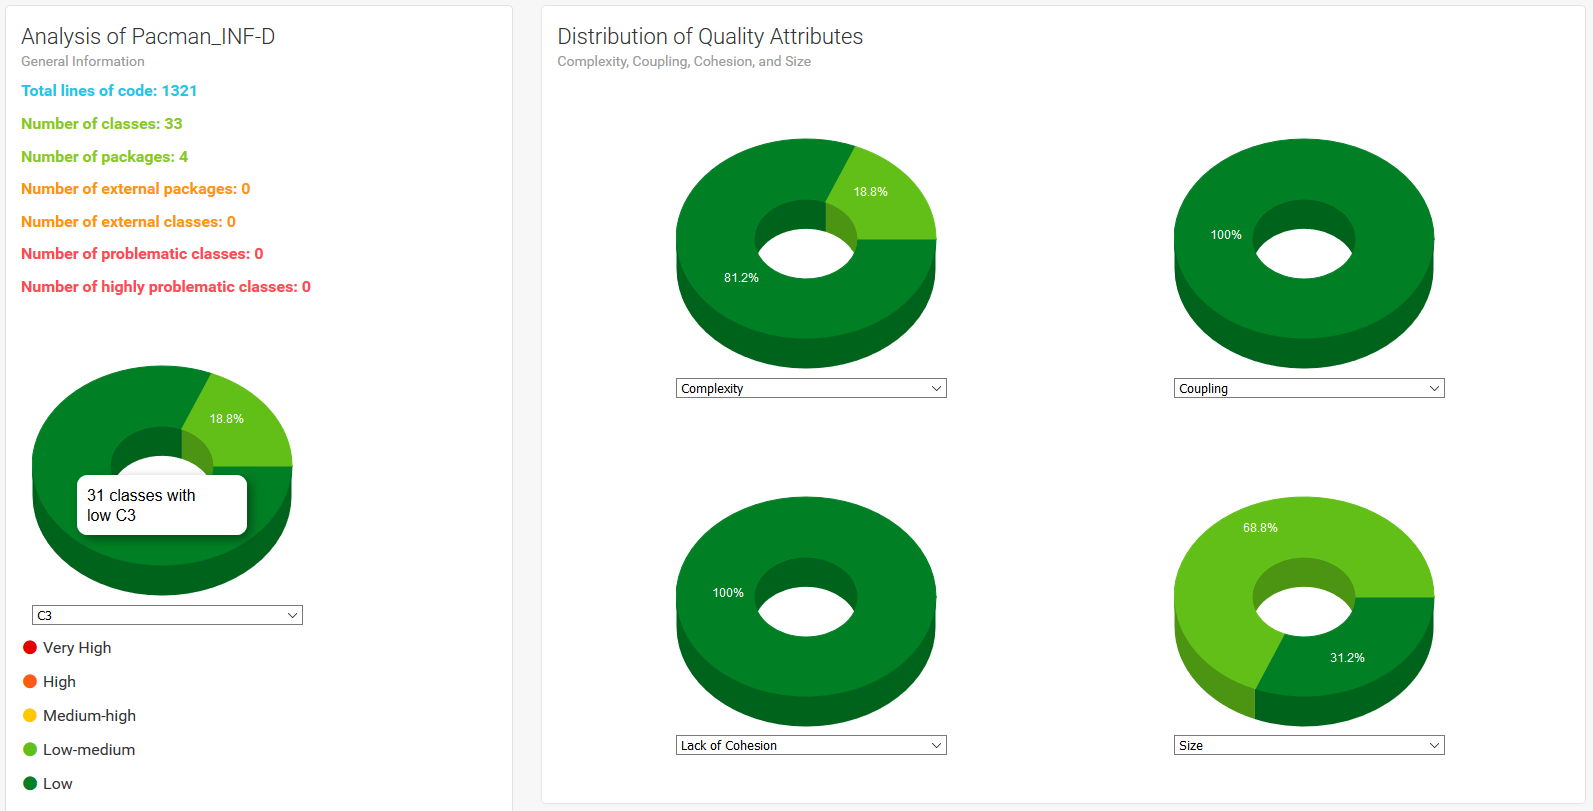
\includegraphics[width=\linewidth]{S3_codeMR_dashboard.png}
\caption{CodeMR dashboard summarizing health of system 3}
\label{fig:S3_codeMR_dashboard}
\end{figure}

\newpage

The \wordlink{Figure}{fig:S3_codeMR_packages} illustrates also the C3 metric but coupled with detailed packages view. We can see that every classes is doing good. 
\vspace{0.2cm}
\begin{figure}[h]
\centering
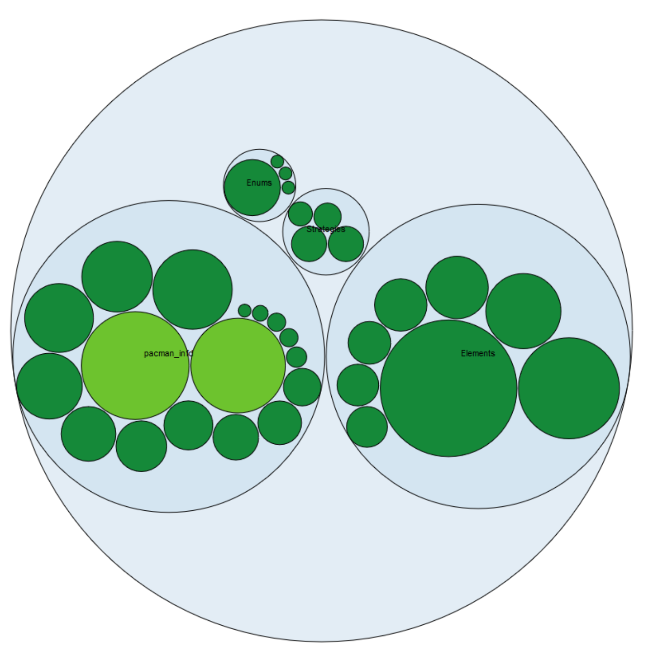
\includegraphics[width=0.8\linewidth]{S3_codeMR_packages.png}
\caption{C3 Metric by package for system 3}
\label{fig:S3_codeMR_packages}
\end{figure}

There are no problems in the classes for almost all the metrics, only for two of them, we can see a problem: the Lack of Tight Class Cohesion  and the lack of Cohesion of Methods. 
For the first one, nine classes have High or Very-High risks like the GameController or the View. And for the latter, three classes have High risks: GameController, ScorePanel and GameWorld.

  
\newpage

\paragraph{Dependencies (CodeMR, Intellij analyzer)}


We use the standard built-in tool of IntellIJ IDEA to analyze the dependency matrix, the result is shown on  \wordlink{Figure}{fig:S3_dep_matrix}. 


\begin{figure}[h!]
\centering
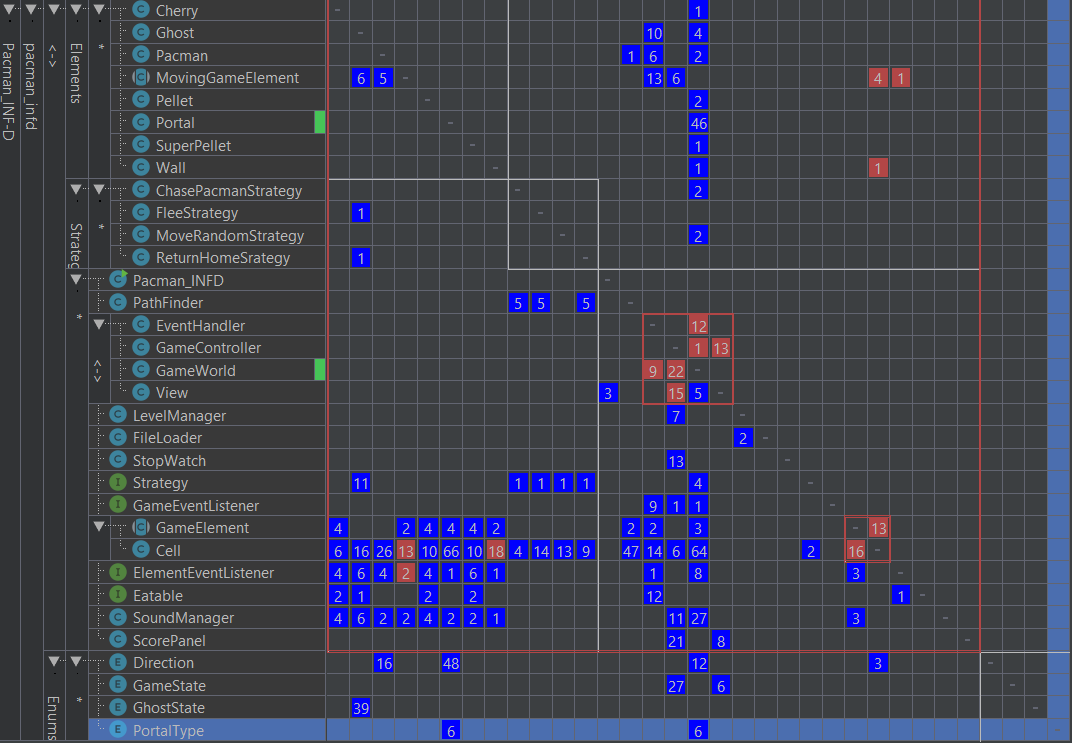
\includegraphics[width=0.8\linewidth]{dependencyM.png}
\caption{Dependency matrix for system 3}
\label{fig:S3_dep_matrix}
\end{figure}

\newpage

\paragraph{Compliance \& bad smells (PMD, Designite)}

We first used PMD, it detected more than 1343 violations in the system 3, here is the result:
\begin{itemize}
    \item 1343 violations: 
    \begin{itemize}
        \item best practice: 54
        \item code style: 414
         \begin{itemize}
            \item 125: method arg could be final 
            \item 98: local var could be final
            \item 60: short variable name
        \end{itemize}
        \item design: 503
        \begin{itemize}
            \item 449: most is law of demeter 'only talk to friends'  
            \item 31: immutable field: private field values never change once object init could be 			                   final
        \end{itemize}
        \item documentation: 192
        \item error prone: 167
        \begin{itemize}
            \item 70: Bean member should serialize: make variable transient or static
            \item 21: avoid literal in if condition
        \end{itemize}
        \item performance: 13
    \end{itemize}
\end{itemize}
		

 The result of Designite analysis is on \wordlink{Figure}{fig:S3_designite}. 

\begin{figure}[h]
\centering
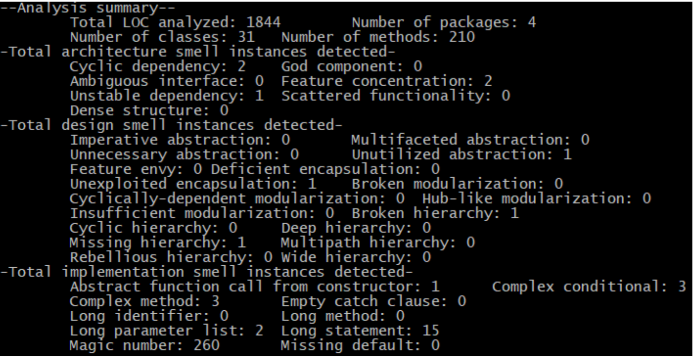
\includegraphics[width=0.85\linewidth]{S3-designite.png}
\caption{Designite in-line use results for system 3}
\label{fig:S3_designite}
\end{figure}


\newpage


\subsubsection{Dynamic Analysis}

\paragraph{Test coverage (Intellij built-in tool)}

The test coverage of the given tests was analyzed, and the three following figures \ref{fig:S3_test_coverage}, \ref{fig:S3_test_coverage0} and \ref{fig:S3_test_coverage2} give the results. We can see that only 28\% of the code is tested and 69\% of the classes. We can see that neither of the strategies in the Strategies packages is tested, and in the Elements package only 12 methods is tested on the 59 methods that are available.


\begin{figure}[h!]
\centering
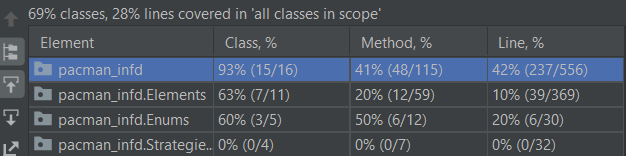
\includegraphics[width=0.75\linewidth]{testCov.png}
\caption{Test coverage for system 3}
\label{fig:S3_test_coverage}
\end{figure}

\begin{figure}[h!]
\centering
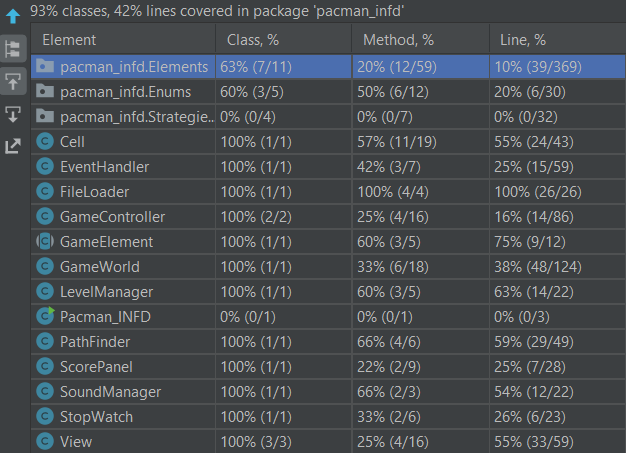
\includegraphics[width=0.75\linewidth]{testCov2.png}
\caption{Test coverage of the pacman\_infd package}
\label{fig:S3_test_coverage0}
\end{figure}

\begin{figure}[h!]
\centering
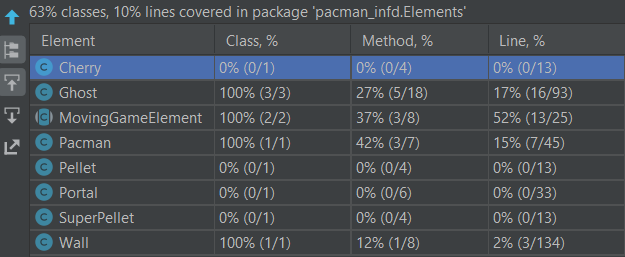
\includegraphics[width=0.75\linewidth]{testCov3.png}
\caption{Test coverage for the Elements package}
\label{fig:S3_test_coverage2}
\end{figure}

\newpage
\clearpage
\section{Quality improvement}

\subsection{System 3 (Robin)}

The first change was changing the building system from Ant to Maven. 
\\

After that, we used PMD and Designite to find problems and refactor them. The access of classes, methods and variables was changed depending of the need, it was set to protected or private if it was possible. Some variables were set to final. We found magic number, and tried to remove them if it was posisble and usefull. 
\\

Then some long methods were divided into multiple methods for more readability. Some switch-case were also added instead of long if-else. Some new method were also added.
\\

The Direction Enumerator class was changed to make it smaller and not just a succesion of switch-case. 
\\

The structure of the classes was also changed. The source code of the project is now divided in 5 packages: Elements, Enums, Fileloader, Game and Strategies. Elements contains all the moving elements of the game, like Pacman or the ghosts, and the other game elements like the cherry or the pellet. The Enums packages contains all the enumeration that are used in the project. The FileLoader package contains all the classes that are used to manage the loading of a level. Strategies contains all the strategies and pathfinders that are used by the ghosts. And the Game package contains everything else that is used for the game, the GameWorld, the Controller or the Listener for exemple.
\\

Then the GUI was changed for Pacman, before changing the code Pacman wasn't changing his orientation on the application, now we can see Pacman change it's orientation. There is also a little animation for the mouth of Pacman, he opens and shut his mouth to simulate eating. 
\\

Some new test where also created on the test package to cover more code. The different strategies of the Strategy package was tested. New tests fot the eating of pellet, cherry and super pellet was also created.
\\




\newpage
\section{Adding basic functionalities}

\subsection{System 3 (Robin)}

In this implementation, we couldn't advance to the next level once we finished eating all the pellets.  We first changed that. Now a level can be succeded and when it's done we advance to the next level, there is 3 level in total but the first 2 are the same.
\\

The levels were also re-writen, in the levels there were some disconnected regions, so we removed that. 
\\

After that the behavior for the super pellet/power pill was also changed. The clock was not set in pause when the pill was activated. The scrone gained by eating the ghosts was also not the one set in the rules, so it was also changed. The time for the pills was also changed, the first two lasts 7 seconds and the last two lasts 5 seconds.
\\

Eating a cherry on the initial implementation wasn't making pacman gain an additional live, so that was also added.


\newpage
\section{Adding new features}
\subsection{System 2 (Robin Schérer)}

Working on this system to implemeent new feature wasn't easy because almost all the logic of the collisions was done in the WorkerProcess class, in this class there is a lot of Feature Envy, this class also have a lot of condition that test the Ghost or Pacman state to see what can happen. \\

This system also doesn't provide a way to change the speed of the DynamicTargets so I had to implement that. The problem is that the run method in WorkerProcess is calling the move function of Pacman on each run, so doing a proper way to handle Target's speed would have needed a lot of refactoring. So I choose to change the REFRESH\_RATE of the run method to 0.1s and the Target has a speed between 0 and 10. At a speed of 0 the target never moves, at 10 the target moves on each run call, at 5 the target moves every 5 call, etc.  \\

In this system the map is really small and adding new element on the map isn't an easy task. I choose that every type of fruits is available at the beginning of the game, just so you can try them, also some more fruit will randomly pop in the board if Pacman has enough score. \\

\begin{figure}[h!]
\centering
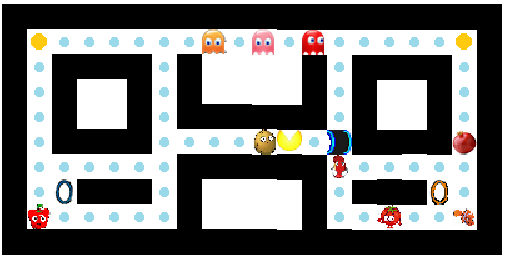
\includegraphics[width=0.75\linewidth]{map.png}
\caption{The system 2 map with the new blocs/fruits}
\label{fig:map}
\end{figure}

The fruits were created using the StaticTarget abstract class as eating a fruit will behave like eating a coin, exept that the eated fruit will trigger a new action. The action will, depending on the fruit, change the way Pacman behave for a certain period of time. Some of the fruits will change Pacman state, like the Bean or the Tomato. \\

\textbf{Fish}  This 'fruit' will make Pacman stops for 3 seconds. It will just change the speed of pacman to 0 for these 3 seconds. \\

\textbf{Grenade} I chose for this fruit to kill every ghosts in a range of 4 blocs and it doesn't care of walls. \\

\textbf{Pepper} The pepper will increase Pacman's speed to the maximum when eaten, so it will be set to 10 for 10 seconds. \\

\textbf{Potato} When eaten, the potato will increase ghost's speed to 7 for 5 seconds. \\

\textbf{Tomato} This fruit will change Pacman's state to INVINSIBLE for 4 seconds, in this mode Pacman cannot be eaten by the ghosts. So as this systems handle collisions in the WorkerProcess I added a condition that the ghost won't eat pacman if he is in this mode. The figure \ref{fig:invisible} shows pacman when he eats this fruit. \\

\begin{figure}[h!]
\centering

\includegraphics[width=0.2\linewidth]{invisible.png}
\caption{Pacman when in invinsible mode}
\label{fig:invisible}
\end{figure}

\textbf{RedBean} This very hot fruit will transform Pacman into Fire mode for 5 seconds, while in this state, he will throw Fireball each time he moves. The fireball kills every Ghost it met and it can cross multiple ghosts. Fireball is implemented with the DynamicTarget abstract class. The figure \ref{fig:fire} shows pacman when in fire mode. \\

\begin{figure}[h!]
\centering

\includegraphics[width=0.2\linewidth]{fire.png}
\caption{Pacman when in fire mode}
\label{fig:fire}
\end{figure}

The new map objects were implemented using a new abstract class that extends the MapObject abstract class. These objects will trigger some action when a Target is on it. \\

\textbf{Trap} This box will make the ghost or pacman's  speed to 0 for 3 seconds, it can only handle 1 target at a time, so if a ghost is stuck on the trap another ghost can cross it. \\

\textbf{Teleporter} There is 2 types of teleporter, an entry and a exit. When created a teleporter will be linked to another teleporter or liked to nothing, if the teleporter has a link it will move Pacman to the exit teleporter. On \wordlink{Figure}{fig:map} we can see the two types of teleporter, the blue on is the entry teleporter and the orange one is the exit. \\

\textbf{Bridge} The bridge can normally be used to make pacman cross crossroads, but in this systems there is none on the map, so in this case it will just block Pacman. For this block I created a new kind of state for DynamicTarget, the bridgeState, this state will have 3 main states: NOT\_ON, UNDER and ON. So it will be used to knwo if a target is not on a bridge, or under/on a bridge, collision between a ghost and pacman that are not on the same state won't happen. The  \wordlink{Figure}{fig:bridgeU} shows Pacman on a bridge and figure \wordlink{Figure}{fig:bridge} 'shows' pacman under a bridge.\\

\begin{figure}[h!]
\centering

\includegraphics[width=0.2\linewidth]{bridge2.png}
\caption{Pacman when on a bridge}
\label{fig:bridgeU}
\end{figure}

\begin{figure}[h!]
\centering

\includegraphics[width=0.2\linewidth]{bridge3.png}
\caption{Pacman when under a bridge}
\label{fig:bridge}
\end{figure}


\section{Quality evolution analysis}
\subsection{System 2 (Robin Schérer)}

\subsubsection{Generalities}

This system is a mess, Rémy improved it but the system was too bad to begin with, everything could have been changed but it would have taken too much time. The way the collisions are handled is, I think, bad, it's not really clear how we have to create new collision type. Also creating or modify the map is dreadful, it was a pain to change the map, but of course changing that would have taken a lot of time. Creating new type of object is also not that easy because we have to create new Containers, ... And WorkerProcess is, in my mind, a mess in general, it doesn't really respect object oriented programming, everything is compared with else-if with a lot of Feature Envy, everything could have been reworked to make it clearer and simpler to update. But still tanks to Rémy this system is clearer than before.

\subsubsection{Static Analysis}
\subsubsection{Code Metrics (CodeMR)}
  CodeMR was used before to anylise the system but now we cannot do it because of the free version, the system is now too big for the free trial. We couldn't afford to buy the full version.

\subsubsection{Compliance & bad smells (PMD, Designite)} 

\textbf{PMD} The \wordlink{Figure}{fig:pmd} shows the results of the PMD analysis, we can see that there is 1880 violations.

\textbf{Designite} The \wordlink{Figure}{fig:designite} shows the results of the Designite analysis, there is still a lot of code smels, like 12 cyclic dependencies, 7 complex method, 1 Feature Envy and 162 magic numbers.

\begin{figure}[h!]
\centering
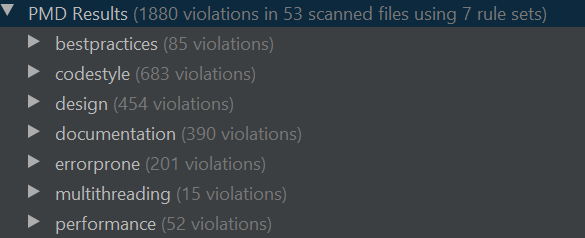
\includegraphics[width=0.75\linewidth]{pmdFinal.png}
\caption{PMD results for system 2}
\label{fig:pmd}
\end{figure}

\begin{figure}[h!]
\centering
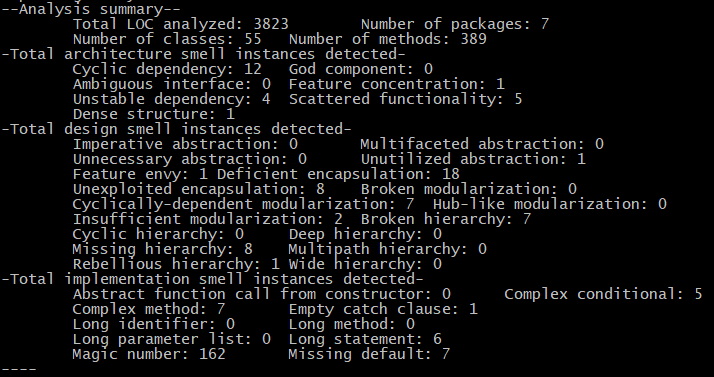
\includegraphics[width=0.75\linewidth]{designiteFinal.png}
\caption{Designite result for system 2}
\label{fig:designite}
\end{figure}

\subsubsection{Test coverage (Intellij built-in tool}

The following figures \ref{fig:acov},  and \ref{fig:acov2} shows the test coverage. All the tests passed and almost all the code is covered. We can see that 96\% of the classes were tested and 71\% of the code line. 

\begin{figure}[h!]
\centering
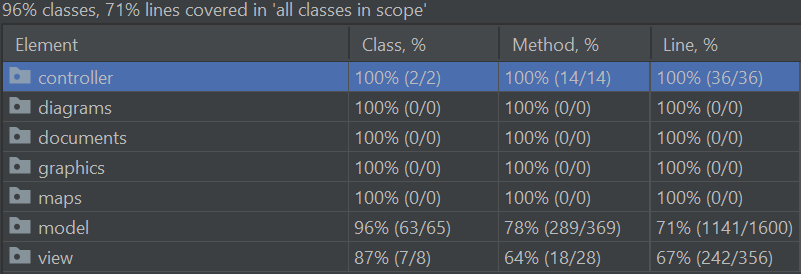
\includegraphics[width=0.75\linewidth]{testCovS2.png}
\caption{System 2 test coverage}
\label{fig:acov}
\end{figure}

\begin{figure}[h!]
\centering
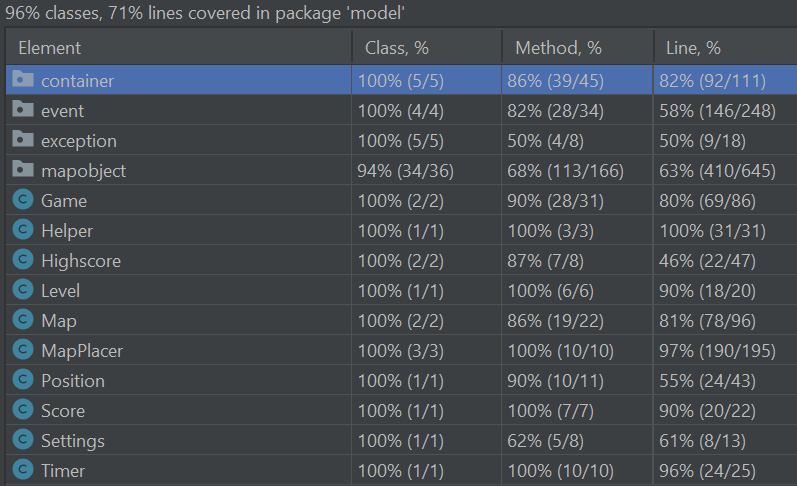
\includegraphics[width=0.75\linewidth]{testCov2S2.png}
\caption{System 2 test coverage}
\label{fig:acov2}
\end{figure}



 
\end{document}